\section{Evaluation} \label{evaluation}

Die Bearbeitung der Forschungsfrage hat folgende Ergebnisse hervorgebracht: Aus ursprünglich 96~924 potenziell relevanten Ufo-Sichtungen im Datensatz konnten für 2~020 Sichtungen zu dem Zeitpunkt passende Wetterdaten gefunden werden, das entspricht ungefähr 2,1\%. Mit welcher Art der drei Vergleichsdaten die Sichtungen analysiert wurden lässt sich in Tabelle \ref{tab:data} ablesen.

\begin{figure}[t]
    \centering
    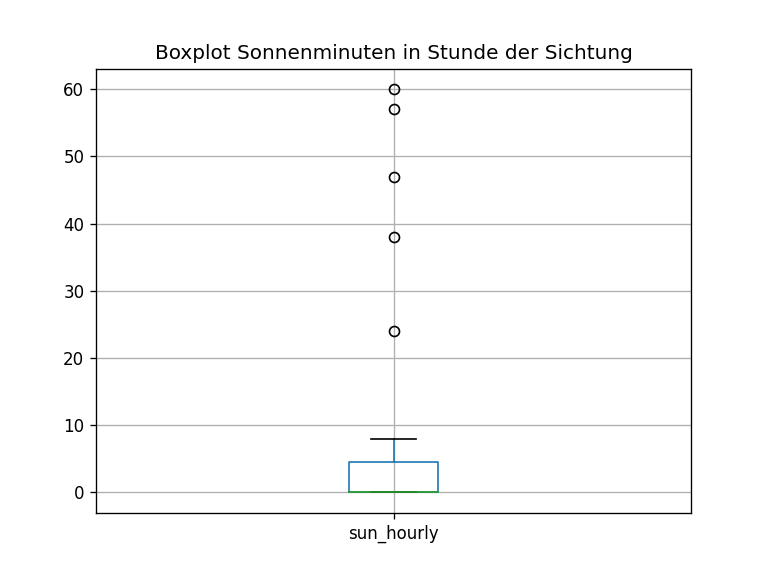
\includegraphics[width=\columnwidth]{hourly_suntime_boxplot}
    \caption{Sonnenminuten pro Stunde.}
    \label{fig:hourly_suntime}
\end{figure}

Die Vergleichsdaten mit dem am Abstand wenigsten Vorkommen bilden die Sonnenminuten pro Stunde mit lediglich 26 Einträgen. Wie in Abbildung \ref{fig:hourly_suntime} zu erkennen ist, befindet sich die Mehrheit davon im Bereich von 0 bis 5 Sonnenminuten pro Stunde. Vereinzelte Ausreißer reichen gegen 50 bis 60 Sonnenminuten.%Aufgrund der sehr geringen Datenmenge und der Erkenntnis, dass es sich bei fast allen Werten um \enquote{0 Minuten} handelt,  

\begin{figure}[t]
    \centering
    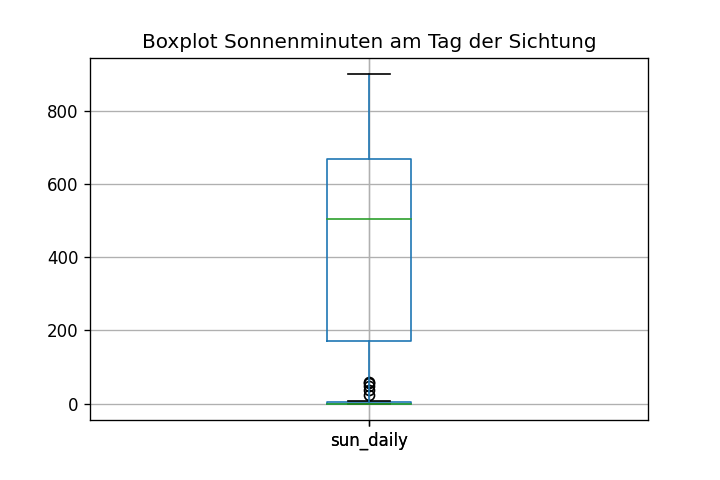
\includegraphics[width=\columnwidth]{daily_suntime_boxplot}
    \caption{Sonnenminuten pro Tag.}
    \label{fig:daily_suntime}
\end{figure}

Abbildung \ref{fig:daily_suntime} beschreibt die Verteilung der Sonnenminuten pro Tag an jeder verfügbaren Ufo-Sichtung. Die mittleren 50\% der Ergebnisse sind hierbei, im Gegensatz zu den stündlichen Sonnenminuten, breiter verteilt. Sie reichen von 200 bis 700 Sonnenminuten pro Tag mit wenigen Ausreißern, welche nur gegen weniger Minuten streben. Im Schnitt scheint die Sonne während eines Tages, an dem ein vermeintliches Ufo gesichtet wurde, um die 500 Minuten -- also etwas mehr als 8 Stunden. In Anbetracht dessen, dass die durchschnittlichen Sonnenstunden in den USA im Bereich zwischen 2 Stunden im Winter und bis zu 12 Stunden im Sommer reichen, kann man den Ufo-Sichtungen eine leichte Überdurchschnittlichkeit an Sonnenstunden zuordnen\cite{statista:2021}.

\begin{table}[t]
    \caption{Condition Codes.}
    \label{tab:coco}
    \centering
    \small
    \begin{tabular}{l l r}
        \toprule
        Code & Weather Condition\cite{coco:2021} & Anzahl\\
        \midrule
        0 & - & 15\\
        1 & Clear & 227\\
        2 & Fair & 603\\
        3 & Cloudy & 363\\
        4 & Overcast & 93\\
        5 & Fog & 186\\
        7 & Light Rain & 219\\
        8 & Rain & 51\\
        9 & Heavy Rain & 9\\
        12 & Sleet & 1\\
        14 & Light Snowfall & 42\\
        15 & Snowfall & 2\\
        16 & Heavy Snowfall & 1\\
        17 & Rain Shower & 9\\
        18 & Heavy Rain Shower & 23\\
        25 & Thunderstorm & 35\\
        26 & Heavy Thunderstorm & 5\\
        27 & Storm & 2\\
        \bottomrule
    \end{tabular}
\end{table}
